\documentclass[11pt]{article}
\usepackage{graphicx}
\usepackage[margin=2.5cm]{geometry}
\usepackage{tikz}
\usepackage{indentfirst}
\usepackage{tabularx}
\usepackage{array}
\usepackage[portuguese]{babel}

\graphicspath{{./images/}}

\def\checkmark{\tikz\fill[scale=0.4](0,.35) -- (.25,0) -- (1,.7) -- (.25,.15) -- cycle;} 
\setlength{\parskip}{0.5em}

\begin{document}
	\begin{titlepage}
	\begin{center}
		
\includegraphics[width=0.6\textwidth]{logo-isec}
		
		\vspace*{\fill}
		
		\Huge
		\textbf{Interação Pessoa-Máquina}
		
		\huge
		Avaliação da Interface de dispositivos
		
		\vspace{0.5cm}
		\LARGE
		2020 - 2021
		
		\vspace{1.5cm}
		
		\textbf{TheForgotten\\merlin-twist}
		
		\begin{figure}[h]
			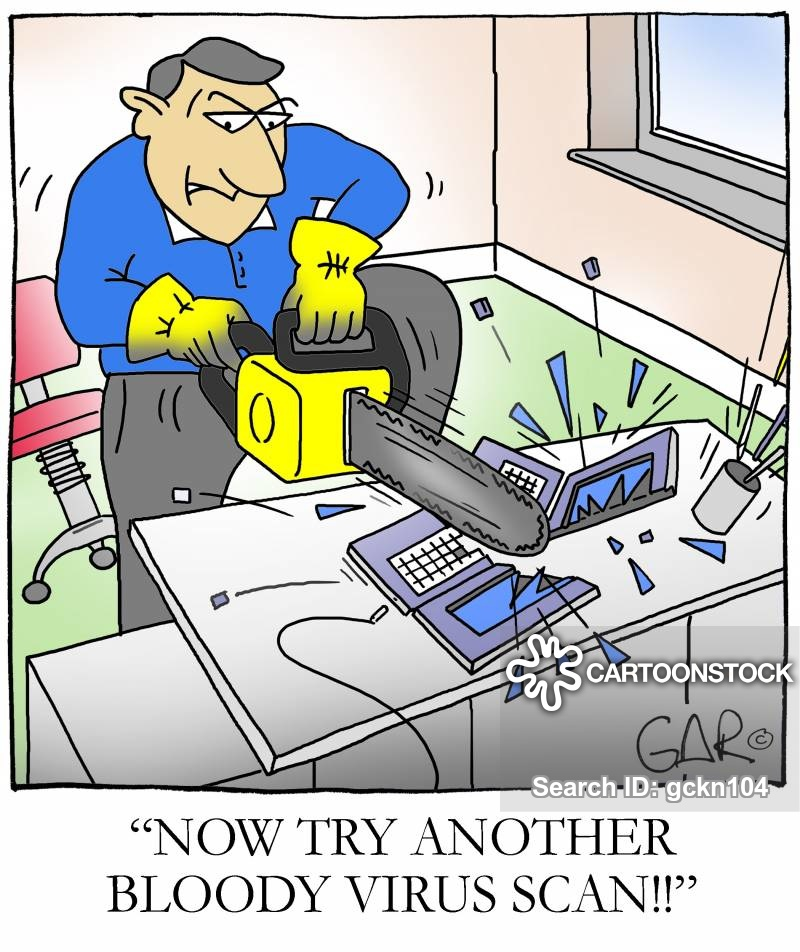
\includegraphics[width=0.5\textwidth]{boomer}
			\centering
			\caption{Homem irritado com o computador}
			\label{fig:angry-man}
		\end{figure}
		
		\vfill
		\vspace*{\fill}
		
		\normalsize
		Licenciatura de Engenharia Informática \\
		5 de março de 2021		
	\end{center}
\end{titlepage}
	
	\tableofcontents
	\pagebreak
	
	\normalsize
	\begin{center}
		\begin{tabularx}{\textwidth}{ |>{\raggedright\arraybackslash}X| }
			\hline
			\textbf{Nome do Produto:} \\ 
			store.kromgaming.com \\ \hline
			\textbf{Data do Estudo:} \\ 
			25 de abril de 2021 \\ \hline
			\textbf{Nomes dos Pesquisadores:} \\ 
			Tomé Madail \\ \hline   
		\end{tabularx}
	\end{center}
	
	\large
	\section{Relatório de Aspeto de Usabilidade}
	
	\normalsize
	\begin{center}
		\begin{tabularx}{\textwidth}{ | >{\raggedright\arraybackslash}X | >{\raggedright\arraybackslash}X | }
			\hline
			\textbf{No.} & \textbf{Problema / Bom aspeto} \\ 
			HE1 & Bom aspeto \\ \hline
			\multicolumn{2}{|l|}{\textbf{Nome:}} \\ 
			\multicolumn{2}{|l|}{Visibilidade dos Indicadores} \\ \hline
			\multicolumn{2}{|l|}{\textbf{Evidência:}} \\ 
			\multicolumn{2}{|l|}{Heurística: H2-1 Visibilidade do sistema} \\
			\multicolumn{2}{|l|}{Onde: páginas todas} \\ 
			\multicolumn{2}{|l|}{} \\ 
			\multicolumn{2}{| >{\hsize=\dimexpr2\hsize+2\tabcolsep+\arrayrulewidth\relax}X |}{Quando o site precisa de carregar algum tipo de informação ou página é nos dado algum tipo de indicador.} \\ \hline  
			\multicolumn{2}{|l|}{\textbf{Explicação:}} \\ 
			\multicolumn{2}{| >{\hsize=\dimexpr2\hsize+2\tabcolsep+\arrayrulewidth\relax}X |}{A heurística é respeitada. O site possui indicadores cada vez que é necessário esperar.} \\ \hline  
			\multicolumn{2}{|l|}{\textbf{Severidade ou benefício:}} \\
			\multicolumn{2}{|l|}{\textbf{Rating:} 0 - não é um problema} \\ 
			\multicolumn{2}{|l|}{\textbf{Justificação:}} \\ 
			\multicolumn{2}{|l|}{\hspace{10mm}\textbf{Frequência:} comum} \\
			\multicolumn{2}{|l|}{\hspace{10mm}\textbf{Impacto:} fácil de superar} \\
			\multicolumn{2}{|l|}{\hspace{10mm}\textbf{Persistência:} persistente} \\
			\multicolumn{2}{| >{\hsize=\dimexpr2\hsize+2\tabcolsep+\arrayrulewidth\relax}X |}{\hspace{10mm}\textbf{Como eu medi os fatores:} sempre que o site demora um bocado a carregar uma informação o utilizador irá ver um indicador. } \\ \hline  
			\multicolumn{2}{|l|}{\textbf{Possíveis soluções e/ou trade-offs:}} \\ 
			\multicolumn{2}{|l|}{-} \\ \hline  
			\multicolumn{2}{|l|}{\textbf{Relações:}} \\ 
			\multicolumn{2}{|l|}{-} \\ \hline  
		\end{tabularx}
	\end{center}
	
	\begin{center}
		\begin{tabularx}{\textwidth}{ | >{\raggedright\arraybackslash}X | >{\raggedright\arraybackslash}X | }
			\hline
			\textbf{No.} & \textbf{Problema / Bom aspeto} \\ 
			HE2 & Bom aspeto \\ \hline
			\multicolumn{2}{|l|}{\textbf{Nome:}} \\ 
			\multicolumn{2}{|l|}{O site utiliza linguagem comum para o utilizador} \\ \hline
			\multicolumn{2}{|l|}{\textbf{Evidência:}} \\ 
			\multicolumn{2}{|l|}{Heurística: H2-2 Correspondência entre o sistema e o mundo real} \\
			\multicolumn{2}{|l|}{Onde: páginas todas} \\ 
			\multicolumn{2}{|l|}{} \\ 
			\multicolumn{2}{| >{\hsize=\dimexpr2\hsize+2\tabcolsep+\arrayrulewidth\relax}X |}{O site possui uma linguagem amigável para o utilizador e segue convenções do mundo real.} \\ \hline  
			\multicolumn{2}{|l|}{\textbf{Explicação:}} \\ 
			\multicolumn{2}{| >{\hsize=\dimexpr2\hsize+2\tabcolsep+\arrayrulewidth\relax}X |}{A heurística é respeitada. O site possui uma linguagem fácil de entender para o utilizador.} \\ \hline  
			\multicolumn{2}{|l|}{\textbf{Severidade ou benefício:}} \\
			\multicolumn{2}{|l|}{\textbf{Rating:} 0 - não é um problema} \\ 
			\multicolumn{2}{|l|}{\textbf{Justificação:}} \\ 
			\multicolumn{2}{|l|}{\hspace{10mm}\textbf{Frequência:} comum} \\
			\multicolumn{2}{|l|}{\hspace{10mm}\textbf{Impacto:} fácil de superar} \\
			\multicolumn{2}{|l|}{\hspace{10mm}\textbf{Persistência:} persistente} \\
			\multicolumn{2}{| >{\hsize=\dimexpr2\hsize+2\tabcolsep+\arrayrulewidth\relax}X |}{\hspace{10mm}\textbf{Como eu medi os fatores:} qualquer utilizador comum consegue entender o que está no site.} \\ \hline  
			\multicolumn{2}{|l|}{\textbf{Possíveis soluções e/ou trade-offs:}} \\ 
			\multicolumn{2}{|l|}{-} \\ \hline  
			\multicolumn{2}{|l|}{\textbf{Relações:}} \\ 
			\multicolumn{2}{|l|}{-} \\ \hline  
		\end{tabularx}
	\end{center}

	\begin{center}
		\begin{tabularx}{\textwidth}{ | >{\raggedright\arraybackslash}X | >{\raggedright\arraybackslash}X | }
			\hline
			\textbf{No.} & \textbf{Problema / Bom aspeto} \\ 
			HE3 & Bom aspeto \\ \hline
			\multicolumn{2}{|l|}{\textbf{Nome:}} \\ 
			\multicolumn{2}{|l|}{Navegação de forma livre} \\ \hline
			\multicolumn{2}{|l|}{\textbf{Evidência:}} \\ 
			\multicolumn{2}{|l|}{Heurística: H2-3 Controlo e liberdade do utilizador} \\
			\multicolumn{2}{|l|}{Onde: todas as páginas} \\ 
			\multicolumn{2}{|l|}{} \\ 
			\multicolumn{2}{| >{\hsize=\dimexpr2\hsize+2\tabcolsep+\arrayrulewidth\relax}X |}{Não obriga o utilizador a caminhos inflexíveis, sendo sempre possível voltar atrás (undo e/ou sair).} \\ \hline  
			\multicolumn{2}{|l|}{\textbf{Explicação:}} \\ 
			\multicolumn{2}{| >{\hsize=\dimexpr2\hsize+2\tabcolsep+\arrayrulewidth\relax}X |}{A heurística é respeitada. O utilizador consegue navegar pelo site de forma livre.} \\ \hline  
			\multicolumn{2}{|l|}{\textbf{Severidade ou benefício:}} \\
			\multicolumn{2}{|l|}{\textbf{Rating:} 0 - não é um problema} \\ 
			\multicolumn{2}{|l|}{\textbf{Justificação:}} \\ 
			\multicolumn{2}{|l|}{\hspace{10mm}\textbf{Frequência:} comum} \\
			\multicolumn{2}{|l|}{\hspace{10mm}\textbf{Impacto:} fácil de superar} \\
			\multicolumn{2}{|l|}{\hspace{10mm}\textbf{Persistência:} persistente} \\
			\multicolumn{2}{| >{\hsize=\dimexpr2\hsize+2\tabcolsep+\arrayrulewidth\relax}X |}{\hspace{10mm}\textbf{Como eu medi os fatores:} quando acontecem situações inesperadas o utilizador consegue sempre voltar atrás sem perder alterações feitas anteriormente.} \\ \hline  
			\multicolumn{2}{|l|}{\textbf{Possíveis soluções e/ou trade-offs:}} \\ 
			\multicolumn{2}{|l|}{-} \\ \hline  
			\multicolumn{2}{|l|}{\textbf{Relações:}} \\ 
			\multicolumn{2}{|l|}{-} \\ \hline  
		\end{tabularx}
	\end{center}
	
	\begin{center}
		\begin{tabularx}{\textwidth}{ | >{\raggedright\arraybackslash}X | >{\raggedright\arraybackslash}X | }
			\hline
			\textbf{No.} & \textbf{Problema / Bom aspeto} \\ 
			HE4 & Problema \\ \hline
			\multicolumn{2}{|l|}{\textbf{Nome:}} \\ 
			\multicolumn{2}{|l|}{Falha de consistência na língua usada} \\ \hline
			\multicolumn{2}{|l|}{\textbf{Evidência:}} \\ 
			\multicolumn{2}{|l|}{Heurística: H2-4 Consistência e aderência a normas} \\
			\multicolumn{2}{| >{\hsize=\dimexpr2\hsize+2\tabcolsep+\arrayrulewidth\relax}X |}{Onde: Publicidades, as páginas “Terms and Conditions”, “Privacy”, “Warranty”, “Shipments” e provavelmente mais algumas.} \\ 
			\multicolumn{2}{|l|}{} \\ 
			\multicolumn{2}{| >{\hsize=\dimexpr2\hsize+2\tabcolsep+\arrayrulewidth\relax}X |}{A língua do site está definida para Inglês, mas mesmo assim, quando aparece uma publicidade ou se acede à página da garantia, as mesmas aparecem em Espanhol.} \\ 
			\multicolumn{2}{| >{\hsize=\dimexpr2\hsize+2\tabcolsep+\arrayrulewidth\relax}X |}{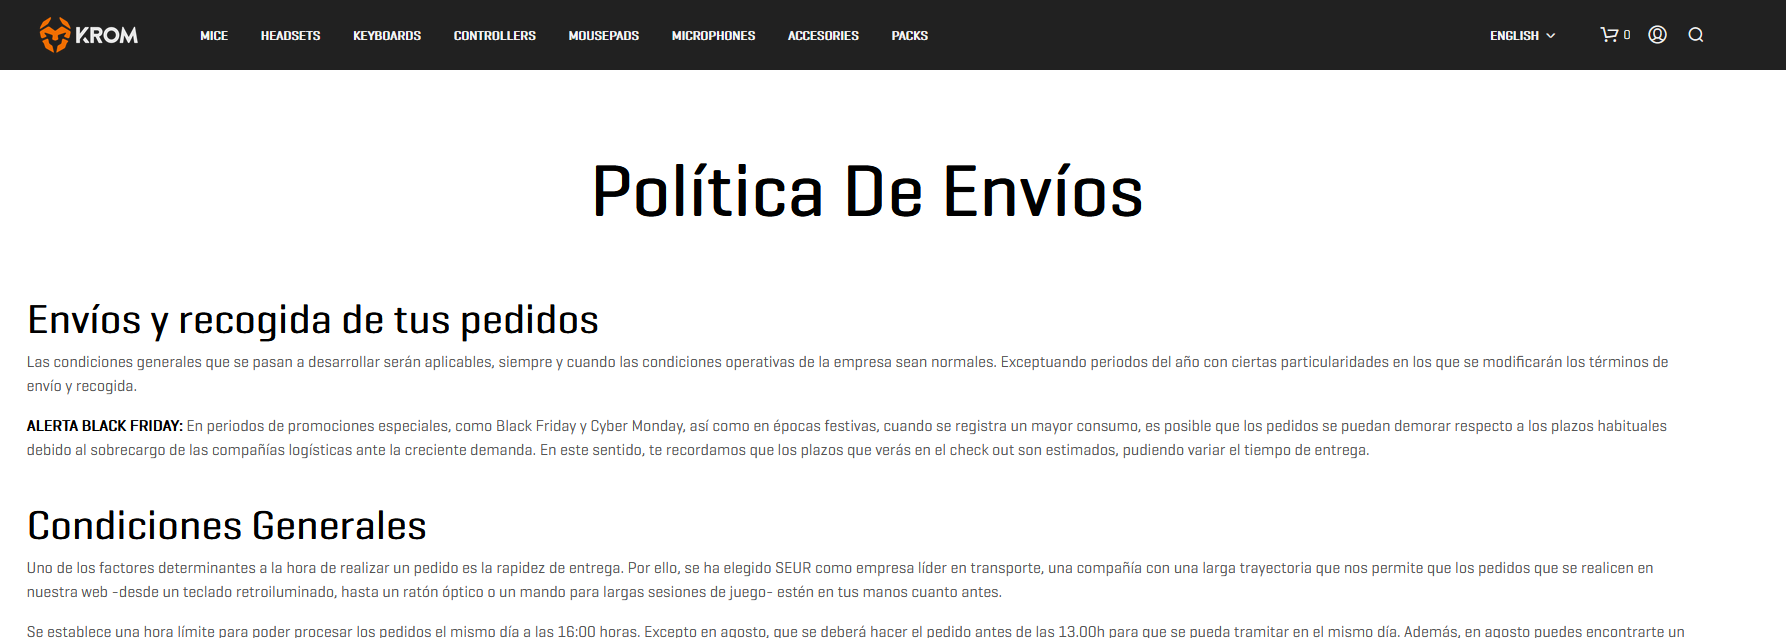
\includegraphics[width=0.9\columnwidth]{politicadeenvios-krom}} \\ \hline
			\multicolumn{2}{|l|}{\textbf{Explicação:}} \\ 
			\multicolumn{2}{| >{\hsize=\dimexpr2\hsize+2\tabcolsep+\arrayrulewidth\relax}X |}{A heurística não é respeitada. O site não utiliza sempre a mesma língua.} \\ \hline  
			\multicolumn{2}{|l|}{\textbf{Severidade ou benefício:}} \\
			\multicolumn{2}{|l|}{\textbf{Rating:} 4 - catástrofe de usabilidade} \\ 
			\multicolumn{2}{|l|}{\textbf{Justificação:}} \\ 
			\multicolumn{2}{|l|}{\hspace{10mm}\textbf{Frequência:} comum} \\
			\multicolumn{2}{|l|}{\hspace{10mm}\textbf{Impacto:} difícil de superar} \\
			\multicolumn{2}{|l|}{\hspace{10mm}\textbf{Persistência:} persistente} \\
			\multicolumn{2}{| >{\hsize=\dimexpr2\hsize+2\tabcolsep+\arrayrulewidth\relax}X |}{\hspace{10mm}\textbf{Como eu medi os fatores:} o utilizador escolhe uma língua para ver o site, mas o site não respeita essa decisão em algumas das páginas e força o utilizador a ver as mesmas em espanhol.} \\ \hline  
			\multicolumn{2}{|l|}{\textbf{Possíveis soluções e/ou trade-offs:}} \\ 
			\multicolumn{2}{|l|}{Fazer a tradução das páginas referidas para as línguas que o site oferece.} \\ \hline  
			\multicolumn{2}{|l|}{\textbf{Relações:}} \\ 
			\multicolumn{2}{|l|}{-} \\ \hline  
		\end{tabularx}
	\end{center}

	\begin{center}
		\begin{tabularx}{\textwidth}{ | >{\raggedright\arraybackslash}X | >{\raggedright\arraybackslash}X | }
			\hline
			\textbf{No.} & \textbf{Problema / Bom aspeto} \\ 
			HE5 & Bom Aspeto \\ \hline
			\multicolumn{2}{|l|}{\textbf{Nome:}} \\ 
			\multicolumn{2}{| >{\hsize=\dimexpr2\hsize+2\tabcolsep+\arrayrulewidth\relax}X |}{Adicionar um produto com um valor abaixo de 1 ao carrinho} \\ \hline
			\multicolumn{2}{|l|}{\textbf{Evidência:}} \\ 
			\multicolumn{2}{|l|}{Heurística: H2-5 Prevenção de Erros} \\
			\multicolumn{2}{|l|}{Onde: todas as páginas} \\ 
			\multicolumn{2}{|l|}{} \\ 
			\multicolumn{2}{| >{\hsize=\dimexpr2\hsize+2\tabcolsep+\arrayrulewidth\relax}X |}{Sempre que se tenta meter um número abaixo de 1 na compra de um produto, o site adiciona 1 unidade ao carrinho ou então faz refresh, não adicionando nada.} \\ 
			\multicolumn{2}{| >{\hsize=\dimexpr2\hsize+2\tabcolsep+\arrayrulewidth\relax}X |}{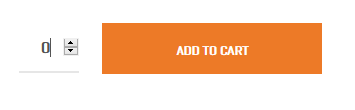
\includegraphics[width=0.5\columnwidth]{addtocart-krom}} \\ \hline
			\multicolumn{2}{|l|}{\textbf{Explicação:}} \\ 
			\multicolumn{2}{| >{\hsize=\dimexpr2\hsize+2\tabcolsep+\arrayrulewidth\relax}X |}{A heurística é respeitada. O site não deixa adicionar produtos com valores negativos.} \\ \hline  
			\multicolumn{2}{|l|}{\textbf{Severidade ou benefício:}} \\
			\multicolumn{2}{|l|}{\textbf{Rating:} 0 - não é um problema} \\ 
			\multicolumn{2}{|l|}{\textbf{Justificação:}} \\ 
			\multicolumn{2}{|l|}{\hspace{10mm}\textbf{Frequência:} comum} \\
			\multicolumn{2}{|l|}{\hspace{10mm}\textbf{Impacto:} fácil de superar} \\
			\multicolumn{2}{|l|}{\hspace{10mm}\textbf{Persistência:} persistente} \\
			\multicolumn{2}{| >{\hsize=\dimexpr2\hsize+2\tabcolsep+\arrayrulewidth\relax}X |}{\hspace{10mm}\textbf{Como eu medi os fatores:} quando se tenta utilizar 0 ou um valor negativo o site por vezes adiciona 1 unidade do item ou então recarrega.} \\ \hline  
			\multicolumn{2}{|l|}{\textbf{Possíveis soluções e/ou trade-offs:}} \\ 
			\multicolumn{2}{| >{\hsize=\dimexpr2\hsize+2\tabcolsep+\arrayrulewidth\relax}X |}{-} \\ \hline  
			\multicolumn{2}{|l|}{\textbf{Relações:}} \\ 
			\multicolumn{2}{|l|}{-} \\ \hline  
		\end{tabularx}
	\end{center}
	
	\begin{center}
		\begin{tabularx}{\textwidth}{ | >{\raggedright\arraybackslash}X | >{\raggedright\arraybackslash}X | }
			\hline
			\textbf{No.} & \textbf{Problema / Bom aspeto} \\ 
			HE6 & Bom aspeto \\ \hline
			\multicolumn{2}{|l|}{\textbf{Nome:}} \\ 
			\multicolumn{2}{| >{\hsize=\dimexpr2\hsize+2\tabcolsep+\arrayrulewidth\relax}X |}{Os produtos de venda são fáceis de identificar} \\ \hline
			\multicolumn{2}{|l|}{\textbf{Evidência:}} \\ 
			\multicolumn{2}{|l|}{Heurística: H2-6 Reconhecer em vez de lembrar} \\
			\multicolumn{2}{|l|}{Onde: páginas todas} \\ 
			\multicolumn{2}{|l|}{} \\ 
			\multicolumn{2}{| >{\hsize=\dimexpr2\hsize+2\tabcolsep+\arrayrulewidth\relax}X |}{Todas as páginas de produtos possuem informação do produto, acompanhada de uma imagem, nome e preço do produto. Ainda diz se existe stock ou não.} \\ 
			\multicolumn{2}{| >{\hsize=\dimexpr2\hsize+2\tabcolsep+\arrayrulewidth\relax}X |}{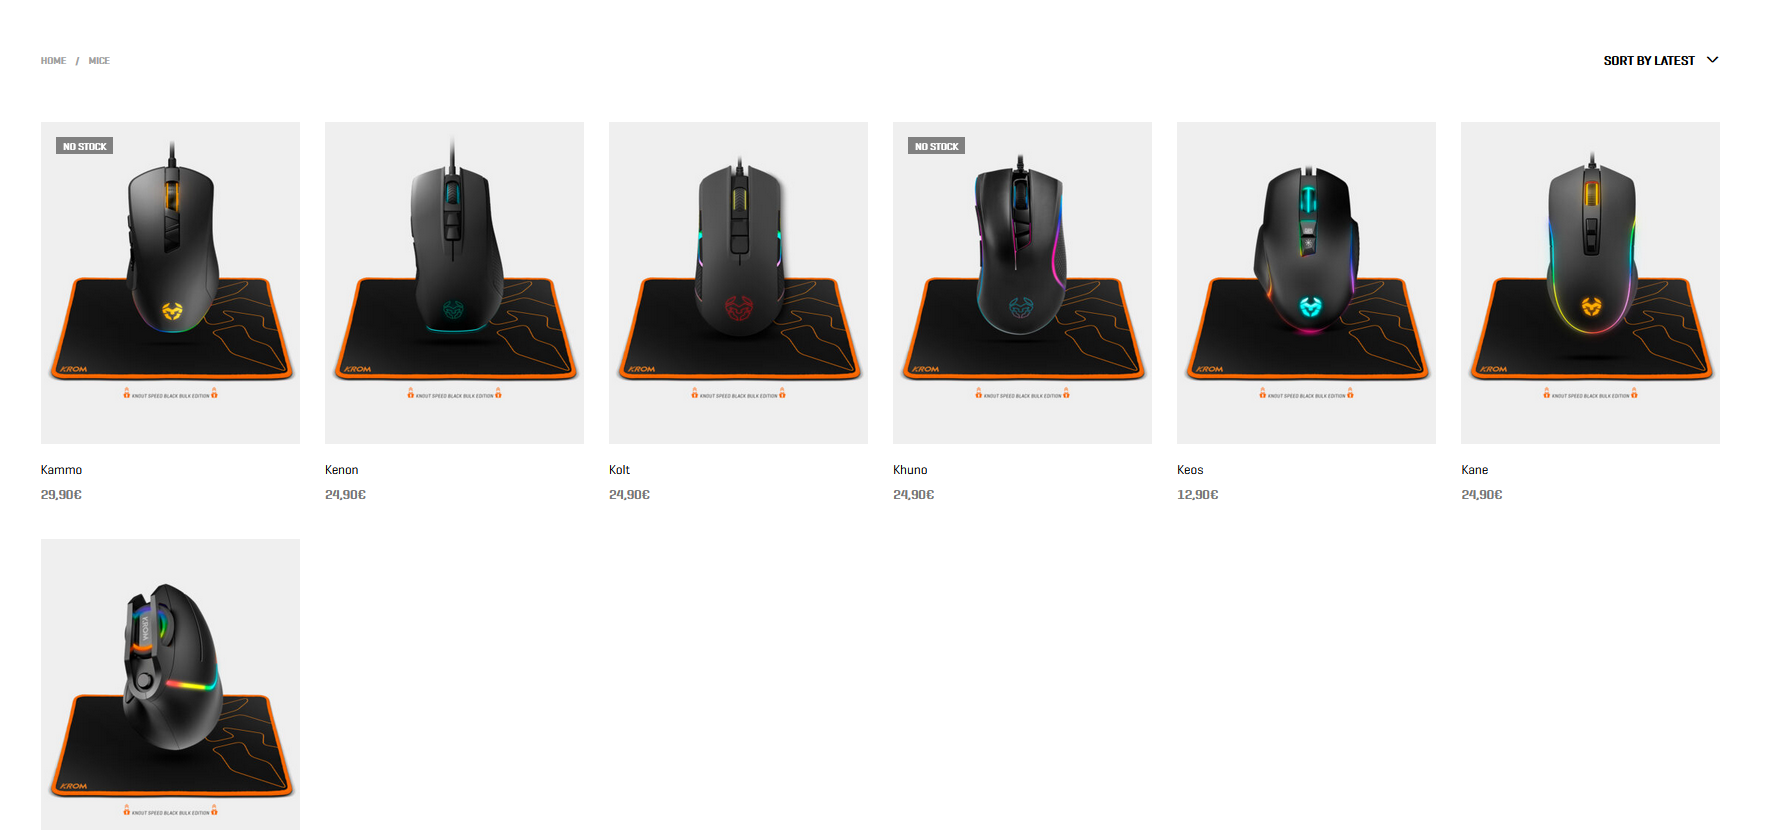
\includegraphics[width=0.9\columnwidth]{mice-krom}} \\ \hline
			\multicolumn{2}{|l|}{\textbf{Explicação:}} \\ 
			\multicolumn{2}{| >{\hsize=\dimexpr2\hsize+2\tabcolsep+\arrayrulewidth\relax}X |}{A heurística é respeitada. O site possui ícones com significado e as ações estão bem identificadas.} \\ \hline  
			\multicolumn{2}{|l|}{\textbf{Severidade ou benefício:}} \\
			\multicolumn{2}{|l|}{\textbf{Rating:} 0 - não é um problema} \\ 
			\multicolumn{2}{|l|}{\textbf{Justificação:}} \\ 
			\multicolumn{2}{|l|}{\hspace{10mm}\textbf{Frequência:} comum} \\
			\multicolumn{2}{|l|}{\hspace{10mm}\textbf{Impacto:} fácil de superar} \\
			\multicolumn{2}{|l|}{\hspace{10mm}\textbf{Persistência:} persistente} \\
			\multicolumn{2}{| >{\hsize=\dimexpr2\hsize+2\tabcolsep+\arrayrulewidth\relax}X |}{\hspace{10mm}\textbf{Como eu medi os fatores:} o utilizador entende sempre o que significa cada imagem e até onde o pode levar.} \\ \hline  
			\multicolumn{2}{|l|}{\textbf{Possíveis soluções e/ou trade-offs:}} \\ 
			\multicolumn{2}{| >{\hsize=\dimexpr2\hsize+2\tabcolsep+\arrayrulewidth\relax}X |}{-} \\ \hline  
			\multicolumn{2}{|l|}{\textbf{Relações:}} \\ 
			\multicolumn{2}{|l|}{-} \\ \hline  
		\end{tabularx}
	\end{center}

	\begin{center}
		\begin{tabularx}{\textwidth}{ | >{\raggedright\arraybackslash}X | >{\raggedright\arraybackslash}X | }
			\hline
			\textbf{No.} & \textbf{Problema / Bom aspeto} \\ 
			HE7 & Bom aspeto \\ \hline
			\multicolumn{2}{|l|}{\textbf{Nome:}} \\ 
			\multicolumn{2}{| >{\hsize=\dimexpr2\hsize+2\tabcolsep+\arrayrulewidth\relax}X |}{O cabeçalho do website possuí bons atalhos} \\ \hline
			\multicolumn{2}{|l|}{\textbf{Evidência:}} \\ 
			\multicolumn{2}{|l|}{Heurística: H2-7 Flexibilidade e Eficiência na utilização} \\
			\multicolumn{2}{|l|}{Onde: páginas todas} \\ 
			\multicolumn{2}{|l|}{} \\ 
			\multicolumn{2}{| >{\hsize=\dimexpr2\hsize+2\tabcolsep+\arrayrulewidth\relax}X |}{O menu possui atalhos para todas as categorias importantes e de lado ainda possui a opção de fazer login, aceder ao carrinho ou fazer uma pesquisa dum produto pelo site.} \\ 
			\multicolumn{2}{| >{\hsize=\dimexpr2\hsize+2\tabcolsep+\arrayrulewidth\relax}X |}{
\includegraphics[width=0.9\columnwidth]{bar-krom}} \\ \hline
			\multicolumn{2}{|l|}{\textbf{Explicação:}} \\ 
			\multicolumn{2}{| >{\hsize=\dimexpr2\hsize+2\tabcolsep+\arrayrulewidth\relax}X |}{A heurística é respeitada. O site possui um bom menu que remete as ações mais frequentes.} \\ \hline  
			\multicolumn{2}{|l|}{\textbf{Severidade ou benefício:}} \\
			\multicolumn{2}{|l|}{\textbf{Rating:} 0 - não é um problema} \\ 
			\multicolumn{2}{|l|}{\textbf{Justificação:}} \\ 
			\multicolumn{2}{|l|}{\hspace{10mm}\textbf{Frequência:} comum} \\
			\multicolumn{2}{|l|}{\hspace{10mm}\textbf{Impacto:} fácil de superar} \\
			\multicolumn{2}{|l|}{\hspace{10mm}\textbf{Persistência:} persistente} \\
			\multicolumn{2}{| >{\hsize=\dimexpr2\hsize+2\tabcolsep+\arrayrulewidth\relax}X |}{\hspace{10mm}\textbf{Como eu medi os fatores:} a utilização do site fica melhor visto que o menu possui atalhos necessários.} \\ \hline  
			\multicolumn{2}{|l|}{\textbf{Possíveis soluções e/ou trade-offs:}} \\ 
			\multicolumn{2}{| >{\hsize=\dimexpr2\hsize+2\tabcolsep+\arrayrulewidth\relax}X |}{-} \\ \hline  
			\multicolumn{2}{|l|}{\textbf{Relações:}} \\ 
			\multicolumn{2}{|l|}{-} \\ \hline  
		\end{tabularx}
	\end{center}

	\begin{center}
		\begin{tabularx}{\textwidth}{ | >{\raggedright\arraybackslash}X | >{\raggedright\arraybackslash}X | }
			\hline
			\textbf{No.} & \textbf{Problema / Bom aspeto} \\ 
			HE8 & Bom aspeto \\ \hline
			\multicolumn{2}{|l|}{\textbf{Nome:}} \\ 
			\multicolumn{2}{| >{\hsize=\dimexpr2\hsize+2\tabcolsep+\arrayrulewidth\relax}X |}{O site possui design apelante e minimalista} \\ \hline
			\multicolumn{2}{|l|}{\textbf{Evidência:}} \\ 
			\multicolumn{2}{|l|}{Heurística: H2-8 Desenho estético e minimalista} \\
			\multicolumn{2}{|l|}{Onde: páginas todas} \\ 
			\multicolumn{2}{|l|}{} \\ 
			\multicolumn{2}{| >{\hsize=\dimexpr2\hsize+2\tabcolsep+\arrayrulewidth\relax}X |}{O site utiliza esquema de cores pouco denso. Não possui botões a mais a atrapalhar a utilização do site.} \\ \hline
			\multicolumn{2}{|l|}{\textbf{Explicação:}} \\ 
			\multicolumn{2}{| >{\hsize=\dimexpr2\hsize+2\tabcolsep+\arrayrulewidth\relax}X |}{A heurística é respeitada. O site é apelante esteticamente.} \\ \hline  
			\multicolumn{2}{|l|}{\textbf{Severidade ou benefício:}} \\
			\multicolumn{2}{|l|}{\textbf{Rating:} 0 - não é um problema} \\ 
			\multicolumn{2}{|l|}{\textbf{Justificação:}} \\ 
			\multicolumn{2}{|l|}{\hspace{10mm}\textbf{Frequência:} comum} \\
			\multicolumn{2}{|l|}{\hspace{10mm}\textbf{Impacto:} fácil de superar} \\
			\multicolumn{2}{|l|}{\hspace{10mm}\textbf{Persistência:} persistente} \\
			\multicolumn{2}{| >{\hsize=\dimexpr2\hsize+2\tabcolsep+\arrayrulewidth\relax}X |}{\hspace{10mm}\textbf{Como eu medi os fatores:} o site utiliza maioritariamente as cores branco, preto e laranja, nunca saindo muito dessa área.} \\ \hline  
			\multicolumn{2}{|l|}{\textbf{Possíveis soluções e/ou trade-offs:}} \\ 
			\multicolumn{2}{| >{\hsize=\dimexpr2\hsize+2\tabcolsep+\arrayrulewidth\relax}X |}{-} \\ \hline  
			\multicolumn{2}{|l|}{\textbf{Relações:}} \\ 
			\multicolumn{2}{|l|}{-} \\ \hline  
		\end{tabularx}
	\end{center}

	\begin{center}
		\begin{tabularx}{\textwidth}{ | >{\raggedright\arraybackslash}X | >{\raggedright\arraybackslash}X | }
			\hline
			\textbf{No.} & \textbf{Problema / Bom aspeto} \\ 
			HE9 & Bom aspeto \\ \hline
			\multicolumn{2}{|l|}{\textbf{Nome:}} \\ 
			\multicolumn{2}{| >{\hsize=\dimexpr2\hsize+2\tabcolsep+\arrayrulewidth\relax}X |}{O site sugere procurar por uma página sempre que acontece um erro de navegação.} \\ \hline
			\multicolumn{2}{|l|}{\textbf{Evidência:}} \\ 
			\multicolumn{2}{|l|}{Heurística: H2-9 Ajudar o utilizador a Reconhecer, Diagnosticar, Recuperar erros} \\
			\multicolumn{2}{|l|}{Onde: páginas todas} \\ 
			\multicolumn{2}{|l|}{} \\ 
			\multicolumn{2}{| >{\hsize=\dimexpr2\hsize+2\tabcolsep+\arrayrulewidth\relax}X |}{Sempre se tenta aceder a uma página que não existe, o site sugere que o utilizador faça uma pesquisa pelo site.} \\ 
			\multicolumn{2}{| >{\hsize=\dimexpr2\hsize+2\tabcolsep+\arrayrulewidth\relax}X |}{
\includegraphics[width=0.9\columnwidth]{404-krom}} \\ \hline
			\multicolumn{2}{|l|}{\textbf{Explicação:}} \\ 
			\multicolumn{2}{| >{\hsize=\dimexpr2\hsize+2\tabcolsep+\arrayrulewidth\relax}X |}{A heurística é respeitada. O site apresenta algumas soluções para eventuais problemas.} \\ \hline  
			\multicolumn{2}{|l|}{\textbf{Severidade ou benefício:}} \\
			\multicolumn{2}{|l|}{\textbf{Rating:} 0 - não é um problema} \\ 
			\multicolumn{2}{|l|}{\textbf{Justificação:}} \\ 
			\multicolumn{2}{|l|}{\hspace{10mm}\textbf{Frequência:} comum} \\
			\multicolumn{2}{|l|}{\hspace{10mm}\textbf{Impacto:} fácil de superar} \\
			\multicolumn{2}{|l|}{\hspace{10mm}\textbf{Persistência:} persistente} \\
			\multicolumn{2}{| >{\hsize=\dimexpr2\hsize+2\tabcolsep+\arrayrulewidth\relax}X |}{\hspace{10mm}\textbf{Como eu medi os fatores:} é raro o site apresentar erros mas quando os mesmo acontecem ele possui uma solução.} \\ \hline  
			\multicolumn{2}{|l|}{\textbf{Possíveis soluções e/ou trade-offs:}} \\ 
			\multicolumn{2}{| >{\hsize=\dimexpr2\hsize+2\tabcolsep+\arrayrulewidth\relax}X |}{-} \\ \hline  
			\multicolumn{2}{|l|}{\textbf{Relações:}} \\ 
			\multicolumn{2}{|l|}{-} \\ \hline  
		\end{tabularx}
	\end{center}

	\begin{center}
		\begin{tabularx}{\textwidth}{ | >{\raggedright\arraybackslash}X | >{\raggedright\arraybackslash}X | }
			\hline
			\textbf{No.} & \textbf{Problema / Bom aspeto} \\ 
			HE10 & Bom aspeto \\ \hline
			\multicolumn{2}{|l|}{\textbf{Nome:}} \\ 
			\multicolumn{2}{| >{\hsize=\dimexpr2\hsize+2\tabcolsep+\arrayrulewidth\relax}X |}{O site tem uma interface de fácil utilização} \\ \hline
			\multicolumn{2}{|l|}{\textbf{Evidência:}} \\ 
			\multicolumn{2}{|l|}{Heurística: H2-10 Documentação e Ajuda} \\
			\multicolumn{2}{|l|}{Onde: todas as páginas} \\ 
			\multicolumn{2}{|l|}{} \\ 
			\multicolumn{2}{| >{\hsize=\dimexpr2\hsize+2\tabcolsep+\arrayrulewidth\relax}X |}{O site não necessita de documentação visto que a sua interface é o standard dos dias de hoje e é muito fácil de entender.} \\ \hline
			\multicolumn{2}{|l|}{\textbf{Explicação:}} \\ 
			\multicolumn{2}{| >{\hsize=\dimexpr2\hsize+2\tabcolsep+\arrayrulewidth\relax}X |}{A heurística é respeitada. Não é necessária ajuda para utilizar as páginas.} \\ \hline  
			\multicolumn{2}{|l|}{\textbf{Severidade ou benefício:}} \\
			\multicolumn{2}{|l|}{\textbf{Rating:} 0 - não é um problema} \\ 
			\multicolumn{2}{|l|}{\textbf{Justificação:}} \\ 
			\multicolumn{2}{|l|}{\hspace{10mm}\textbf{Frequência:} comum} \\
			\multicolumn{2}{|l|}{\hspace{10mm}\textbf{Impacto:} fácil de superar} \\
			\multicolumn{2}{|l|}{\hspace{10mm}\textbf{Persistência:} persistente} \\
			\multicolumn{2}{| >{\hsize=\dimexpr2\hsize+2\tabcolsep+\arrayrulewidth\relax}X |}{\hspace{10mm}\textbf{Como eu medi os fatores:} navegação intuitiva.} \\ \hline  
			\multicolumn{2}{|l|}{\textbf{Possíveis soluções e/ou trade-offs:}} \\ 
			\multicolumn{2}{| >{\hsize=\dimexpr2\hsize+2\tabcolsep+\arrayrulewidth\relax}X |}{-} \\ \hline  
			\multicolumn{2}{|l|}{\textbf{Relações:}} \\ 
			\multicolumn{2}{|l|}{-} \\ \hline  
		\end{tabularx}
	\end{center}
	
	\large
	\section{Conclusão}
	
	\normalsize
	Com a avaliação deste site conseguimos perceber que o mesmo respeita quase sempre as 10 Heurísticas de Usabilidade (revistas).
\end{document}